\part{Design}
In the previous sections we have discussed and analysed different solutions to the requirements presented in the first part, under section \ref{Requirements}. We will now proceed with describing the implementation of the system and outline the features that fulfils the requirements.

\section{System Flow}
To let the reader get a feel of the system at hand, we will in this section present different diagrams, with associated descriptions, which should improve the readers overall understanding of the system.
As with many others systems, the user has to log in to get full access. As mentioned, we have chosen to use Facebook services, to assist with the login process. It is possible for the user, to get different lists of videos, but for any other service request, the user must login. To do this, the client has to pass a valid Facebook token to the server, which uses this token to contact Facebook, and extract the data needed to create the user in the system. The sequence is illustrated below:

\begin{figure}[H]
\centering
\includegraphics[scale=0.35]{loginWithFacebook.jpg}
\label{loginwithfacebook}
\caption{Sequence diagram of the LoginWithFacebook operation}
\end{figure}


The call issued from the service, results in several calls to Facebook being made. The first one validates the application, meaning the RentIt server contacts Facebook and obtains the id of the app that was used to issue the token. This step is necessary because anyone can in theory register as a Facebook developer and obtain Facebook tokens and use them to access the server. By getting the id of the app that issued the token, we can verify that it was issued by an app that is trusted by the RentIt service, i.e the SMU client or the ITU client.

Next, the users information is validated by retrieving it from Facebook. If the user has not granted the issuing app access to the needed data, the service returns a HTTP error status code to the client. If on the other hand all goes well, the user is added to the database, and added to a datastructure that can then later be used to check if the user is logged in.
After the user is authenticated correctly he is able to use most of the exploited services at the WCF. An example of this is showed at the diagram below:

\begin{figure}[H]
\centering
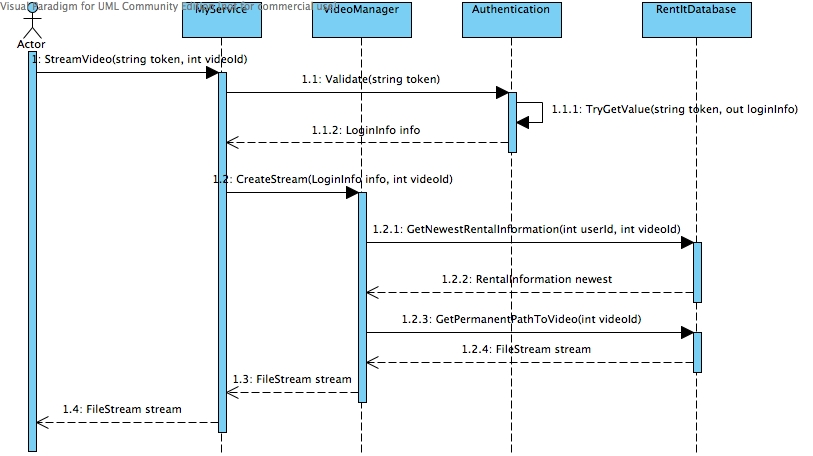
\includegraphics[scale=0.35]{StreamVideo.jpg}
\label{streamvideo}
\caption{Sequence diagram of the StreamVideo operation}
\end{figure}

This shows the flow for the operation for 'StreamVideo'. First the user is validated, using the datastructure that contains all logged in users. If the user is logged in, a check is made to see if the user has an active rent period for the requested video. If this is the case, a stream of video data is returned to the client, otherwise a HTTP error is returned.
